\documentclass[a4paper]{article}
\usepackage[utf8]{inputenc}
\usepackage[spanish]{babel}
\usepackage{graphicx}
\begin{document}
\title{Procesamiento de textos con \LaTeX.}
\author{Tiffany López Nicholson. \\
Técnicas experimentales.}
\date{\today}
\maketitle
\begin{abstract}
	El objetivo de este artículo es explicar como procesar 
	textos en \LaTeX, con el apoyo de lo que se ha dado en clase.	
\end{abstract}
\section{Cómo procesar textos en \LaTeX.}
	\LaTeX{} es una herramienta informática que permite la creación de documentos con imágenes, diferentes tipos de letra, etc. Además según Leslie Lamport, \LaTeX{} es un conjunto de plantillas, patrones o macros de TeX\footnote{TeX es un procesador de textos de alta calidad que contiene muchas expresiones matemáticas.\cite{2}}.
	\subsection{Ventajas.}
	Se crean textos de alta calidad que son independientes de la plataforma. Tiene un diseño  especial para los textos científicos.
	\subsection{¿Cómo trabaja?}
	Primero necesitamos un editor de texto plano, como por ejemplo el bloc de notas. Luego, debemos guardar el fichero con extensión .tex.\par
Para compilarlo escribimos en nuestra consola ''latex ''nombre-del-fichero''.tex''. Se generaran diferentes archivos, el que más nos importa es el fichero ''.dvi''.\par
Para visualizarlo escribimos ''xdvi ''nombre-del-fichero''.dvi''.
\section{Comandos \LaTeX.}
	\subsection{El preámbulo de nuestro texto.}
\begin{figure}
\begin{center}
\includegraphics[width=0.5\textwidth]{pant.eps}
\caption{\small Esto es un ejemplo de cómo empezar nuestro texto.}
\end{center}
\end{figure}
	
Como observamos en la imagen debemos especificar el tamaño de papel que queremos usar, en qué idioma estamos escribiendo, tamaño de la letra, si queremos incluir imágenes... En el ejemplo, se ha especificado en \verb|\documentclass[a4paper]{article}| que nuestra hoja sea DinA4 y el tipo de texto sea un artículo. En \verb|\usepackage[utf8]{inputenc}|
\verb|\usepackage[spanish]{babel}| estamos especificando el idioma; en este caso en espa\~nol. (Ver imagen 1)

	\subsection{Comandos generales.}
	Para crear una tabla deberemos utilizar el comando \verb|begin{tabular} - end{tabular}|.
\begin{table}
\begin{tabular}{|l|c|}
\hline
ALUMNO & NOTA \\ \hline
Alumno 1 & 8 \\ \hline
Alumno 2 & 4 \\ \hline
Alumno 3 & 1 \\ \hline
\end{tabular}
\caption{\textbf{Esto es un ejemplo.}}
\end{table}
	Dentro de esos comandos deberemos escribir los nombres de los diferentes cuadros con un espacio y \verb|&|. Para formar las líneas horizontales debemos escribir \verb|\hline|.

\begin{thebibliography}{00}
	\bibitem{1}
		Di Martino, Matías.
		\emph{CódigoMatu},
		(2009)
	\bibitem{2}
		CTAN.
		\emph{www.ctan.org},
\end{thebibliography}
\end{document}
